%Dokumentinnstillinger:---------------------------------
%Ved å google flitting kan du finne ut hva de forskjellige tingene her betyr, og hvordan du kan gjøre eventuelle endringer.
\documentclass[a4paper,11pt,norsk]{article}
\usepackage[utf8]{inputenc}
\usepackage{a4wide}
\usepackage{lmodern}
\usepackage[T1]{fontenc}
\usepackage{babel}
\setlength{\parindent}{0pt} 
\setlength{\parskip}{2ex}
\usepackage{fixltx2e}
\usepackage{amsmath}
\usepackage[pdftex, pdfborderstyle={/S/U/W 0}]{hyperref}
\usepackage{graphicx}
\usepackage[font=small,labelfont=bf]{caption}
\usepackage{tabularx}
\usepackage{multirow}
\usepackage{tikz}
\usepackage[european]{circuitikz}
\usetikzlibrary{shapes.geometric, arrows}
\tikzstyle{startstop} = [rectangle, rounded corners, minimum width=2.5cm, minimum height=1cm,text centered, draw=black, fill=red!30]
\tikzstyle{io} = [trapezium, trapezium left angle=70, trapezium right angle=110, minimum width=2.5cm, minimum height=1cm, text centered, draw=black, fill=blue!30]
\tikzstyle{process} = [rectangle, minimum width=2.5cm, minimum height=1cm, text centered, draw=black, fill=orange!30]
\tikzstyle{arrow} = [thick,->,>=stealth]
\usepackage{floatrow}
\floatsetup[table]{capposition=top}
% \usepackage[europeanresistors]{circuitikz}
\tikzset{opampdownlbl/.style={
            below,
            draw=none,
            append after command={
                (\tikzlastnode.north) edge ([shift={(-5pt,0pt)}]\tikzlastnode.north) edge ([shift={(+5pt,0pt)}]\tikzlastnode.north)
            }},
        opampuplbl/.style={
            above,
            draw=none,
            append after command={
                (\tikzlastnode.south) edge ([shift={(-5pt,0pt)}]\tikzlastnode.south) edge ([shift={(+5pt,0pt)}]\tikzlastnode.south)
            }}}

% roman numerals
\newcommand{\RNum}[1]{\uppercase\expandafter{\romannumeral #1\relax}}
\usepackage{csquotes}
\usepackage{url}
\usepackage{siunitx}
\usepackage{dirtytalk}
\usepackage{booktabs} % Denne pakken gir tilgang på endel ekstra kommandoer som legger til rette for god skikk og bruk i tabellformatering.
\usepackage{multirow}
\usepackage[font=small,labelfont=bf]{caption}	% Justering av LaTeX standarder for figurtekst og tabelltekst.

\begin{document}

%Headingdel:---------------------------------------------
\begin{minipage}[c]{0.15\textwidth}

\includegraphics[width=2.0cm]{elsys_pos_staaende_ntnu}  
\end{minipage}
\begin{minipage}[c]{0.85\textwidth}

\renewcommand{\arraystretch}{1.7}
\large 
\begin{tabularx}{\textwidth}{|X|X|}
\hline
\multicolumn{2}{|l|}{} \\
\multicolumn{2}{|l|}{\huge \textbf{Designnotat}} \\
\multicolumn{2}{|l|}{}  \\
\hline
\multicolumn{2}{|l|}{Tittel: 
%Skriv inn tittel her:------------------------------------------
Bufferkrets
} \\
\hline
\multicolumn{2}{|l|}{Forfattere: 
%Skriv inn forfattere her:--------------------------------------
Mia Elisenberg
} \\
\hline
%Skriv inn versjon og dato her her:-----------------------------
Versjon: 2.0 & Dato: \today
\\
\hline 
\end{tabularx}
\end{minipage}
\normalsize

%Automatisk generert innholdsfortegnelse:------------------

\setlength{\parskip}{0ex}
\renewcommand{\baselinestretch}{0.1}\normalsize
\tableofcontents
\renewcommand{\baselinestretch}{1.00}\normalsize
\setlength{\parskip}{2ex}
\rule{\textwidth}{1pt}


\newpage

%Selve rapporten:------------------------------------------

\section{Problembeskrivelse}
\label{sec:innledning}

En utfordring i et system kan være at en signalkilde ikke klarer å levere nok strøm til en last. Det kan hende at spenningsnivået er høyt nok, men strømstyrken er ikke nok til å levere effekten lasten krever. En løsning på dette problemet er å bruke en buffer. Konseptet for et slikt system vises i figuren under.

\vspace{1cm}
\begin{figure}[!h]
    \centering
    \begin{circuitikz} [american voltages]
    \draw
    (0,1) to (0,0) node[ground]{}
    (0,2) to [V=$v_0$] (0,1)
    (0,2) to (0,3)
    
    (0,3) to [R, l^=$R_\text{K}$] (3,3)
    
    (3,3) to [short, -*] (4,3)
    (4,3.5) node[]{$v_1$}
    
    (4,3) to (5.5,3)
    (6,3) node[buffer]{}
    
    (6.5,3) to [short, -*] (7.5,3)
    (7.5,3.5) node[]{$v_2$}
    
    (7.5,3) to [short,-] (10,3)
    (10,3) to [R, l^=$R_\text{L}$] (10,0.5)
    
    (10,0.5) to (10,0) node[ground]{}
    ;
    \end{circuitikz}
    \caption{En bufferkrets med en kilde, buffer og last.}
    \label{fig:01}
\end{figure}
\vspace{1cm}

Systemet i figur \ref{fig:01} har en spenningskilde $v_0$, en utgangsmotstand $R_\text{K}$ for kilden, en last $R_\text{L}$ og en buffer med inngangssignal $v_1$ og utgangssignal $v_2$. Bufferen må være slik at

\begin{equation}
    v_2 \approx v_1 \approx v_0
\end{equation}

og den må være mest mulig uavhengig av $R_\text{K}$ og $R_\text{L}$ for å gi et presist resultat.\clearpage
\section{Prinsipiell løsning}
\label{sec:prinsipielllosning}

Det er designet et system ved hjelp av diskrete komponenter for å gjøre resultatet av bufferen så presist som mulig, og kretstopologien vises i figur \ref{fig:02}. Den baserer seg på en NPN-transistor og skal konfigures slik at inngangsmotstanden er høy, og utgangssmotstanden er lav. Dette gjør at systemet kan ha en stor last og en inngangskilde som har en større eller ikke ideell utgangssmotstand. Forsterkningsfaktoren til systemet er tilnærmet lik 1, som vil si at inngangssignalet er tilnærmet lik utgangssignalet, og man har en buffer.

\vspace{1cm}
\begin{figure}[!h]
    \centering
    \begin{circuitikz} [american voltages]
    \draw
    % (0,0) to [short,*-] (1,0)
    (0,0.5) node[]{$v_1$}
    
    (0,0) to [C, l^=$C_1$, *-*] (3,0)
    
    % (2,0) to [short,-*] (3,0)
    
    (3,0) to [R,l^=$R_{\text{B}1}$] (3,3)
    (3,3) to [short,-*] (10,3)
    (10,3.5) node[]{$V_{\text{CC}}$}
    
    (3,0) to [R,l_=$R_{\text{B}2}$] (3,-3)
    (3,-3) to [short,-*] (0,-3)
    
    (3,0) to [short,-*] (4.5,0)
    (4.5,0.5) node[]{$V_\text{B}$}
    
    (4.5,0) to (5.5,0)
    (6,0) to node[npn] (npn) {} (6,0)
    
    (6,0.6) to [short,-*] (6,1)
    (5.5,1) node[]{$V_\text{C}$}
    (6,1) to (6,3)
    
    (6,-0.6) to [short,-*] (6,-1)
    (5.5,-1) node[]{$V_\text{E}$}
    (6,-1) to [R,l_=$R_\text{E}$] (6,-3)
    
    (6,-1) to [C, l^=$C_2$, -*] (10,-1)
    (10,-0.5) node[]{$v_2$}
    
    (3,-3) to [short,-*] (10,-3)
    
    (5,-3) to (5,-3.5) node[ground]{}
    ;
    \end{circuitikz}
    \caption{Kretstopologien til en buffer basert på en NPN-transistor.}
    \label{fig:02}
\end{figure}
\vspace{1cm}

Bufferkretsen i figur \ref{fig:02} består av $v_1$ og $v_2$ som i figur \ref{fig:01} og en forskyningsspenning $V_{\text{CC}}$, i tillegg til motstandene $R_{\text{B}1}$, $R_{\text{B}2}$ og $R_\text{E}$ og kondensatorene $C_1$ og $C_2$.

For å bestemme komponentverdiene, så må en først bestemme verdien av $V_{\text{CC}}$. En kan så styre spenningsfallet over transistorens base. Transistoren vil kunne svinge mellom $V_{\text{CC}}$ og terskelspenninga $V_\text{T}$. Ved å la base-spenninga $V_\text{B}$ være middelverdien av dette, så vil en oppnå mest mulig svingning for $v_1$. Med hensyn til $V_\text{T}$, så vil dette være

\begin{equation}
    V_\text{B} = \frac{(V_{\text{CC}}-V_\text{T})}{2}+V_\text{T}
\end{equation}\label{eq:V_B}

Verdien av $V_\text{B}$ er også gitt av en spenningsdeler bestående av $R_{\text{B}1}$ og $R_{\text{B}2}$, og ved å selv bestemme en verdi av $R_{\text{B}2}$, så får en at verdien til $R_{\text{B}1}$, er gitt ved

\begin{equation}
    V_\text{B} = \frac{R_{\text{B}2}}{(R_{\text{B}1}+R_{\text{B}2})}V_{\text{CC}} \implies R_{\text{B}1} = \frac{V_{\text{CC}}R_{\text{B}2}}{V_\text{B}}-R_{\text{B}2}
\end{equation}\label{eq:R_B1}

Det er viktig å ha en korrekt verdi for $R_\text{E}$ for å forhindre at transistoren overopphetes. En velger en trygg verdi for strømmen $I_\text{E}$ gjennom transistorens emitter, slik at overoppheting ikke skjer. Ved å så bruke Ohms lov, så finner en at

\begin{equation}
    V_\text{E} = R_\text{E}I_\text{E} \implies R_\text{E}=\frac{V_\text{E}}{I_\text{E}} = \frac{(V_\text{B}-V_\text{T})}{I_\text{E}}
\end{equation}\label{eq:R_E}

Både $C_1$ og $C_2$ vil blokkere DC-signaler og kun la AC-signaler komme gjennom. Disse trenger kun å være tilstrekkelig store.\clearpage
\section{Realisering, test og diskusjon}
\label{sec:realisering}

En bruker den bipolare transistoren BC457. Tabell \ref{tab:vars} viser variabelverdier funnet i databladet til transistoren og beregna verdier, slik at transistorens arbeidspunkt skal oppfylles. Fullstendige utregninger finnes i vedlegg \ref{ax:math}.

\vspace{1cm}
\begin{table}[!h]
\centering % Denne kommandoen sentrerer tabellen i kolonnen. 
\caption{Beregna verdier.}
\label{tab:vars}	% Merkelappen vi vil referere til.
\begin{tabular}{lll} % Her angir det andre argumentet at vi vil ha to senterjusterte kolonner (l = left, c = center, r = right).
\toprule % Horisontal linje som markerer toppen av tabellen
\textbf{Variabel/komponent} & \textbf{Verdi} & \textbf{Kommentar} \\
\midrule
$V_{\text{CC}}$ & $6\text{V}$ & \\
$V_\text{T}$ & $0.7\text{V}$ & \\
$R_{\text{B}2}$ & $470\text{k}\Omega$ & inngangsimpedansen må være høy i en buffer \\
$I_\text{E}$ & $10\text{mA}$ & \\
$V_\text{B}$ & $3.35\text{V}$ & \\
$R_{\text{B}1}$ & $690\text{k}\Omega$ & \\
$R_\text{E}$ & $330\Omega$ & utgangsimpedansen er lav i en buffer \\
$C_1$ & $1\mu\text{F}$ & \\
$C_2$ & $1\mu\text{F}$ & \\
\bottomrule 
\end{tabular}
\end{table}
\vspace{1cm}
\clearpage

\subsection{Test under ideelle forhold}
Ved ideelle forhold, så er $R_\text{K}=0$ og $R_\text{L}=\infty$. Inngangssignalet er et sinussignal med frekvens $f=1000\text{Hz}$ og amplitude $A_0=500\text{mV}$. Resultatet vises i figur \ref{fig:ideal}, hvor test-inngangssignalet er $v_1$, og utgangssignalet er $v_2$.

\vspace{1cm}
\begin{figure}[!h]
    \centering
    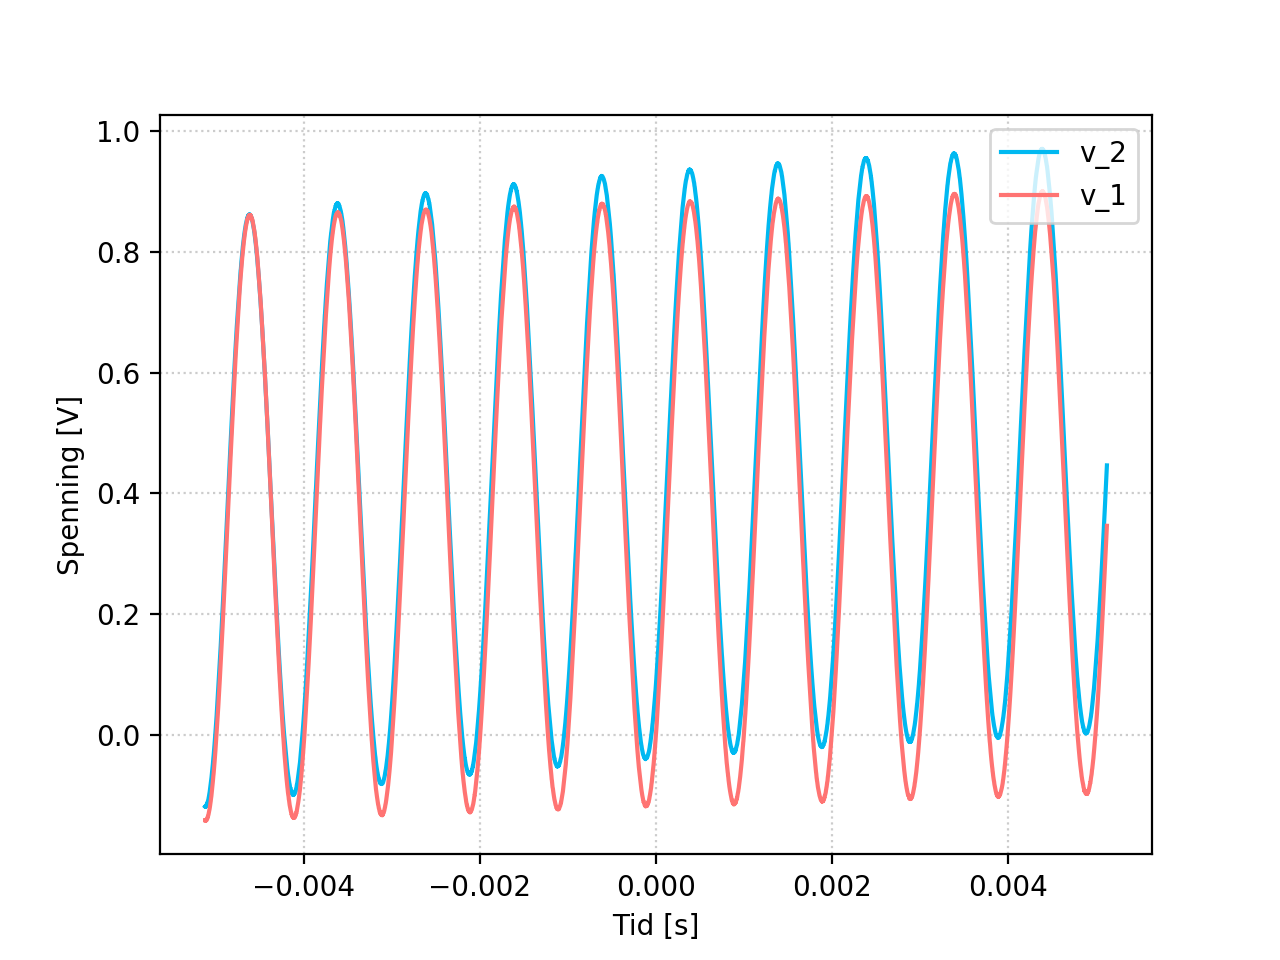
\includegraphics[width=0.8\textwidth]{img/esda2-d5-ideelle-plot.png}
    \caption{Systemet under ideelle forhold.}
    \label{fig:ideal}
\end{figure}
\vspace{1cm}

Amplituden til $v_1$ er $A_1=490\text{mV}$, og amplituden til $v_2$ er $A_2=470\text{mV}$. En ser at $v_2\approx v_1$, som vil si at systemet fungerer godt, men har noe forbedringspotensiale. 

\clearpage

\subsection{Test med reell last og kilde}
En lar $R_\text{L}=220\Omega$ og $R_\text{K}=3.3\text{k}\Omega$. Resultatet av denne addisjonen til systemet vises i figur \ref{fig:real}.

\vspace{1cm}
\begin{figure}[!h]
    \centering
    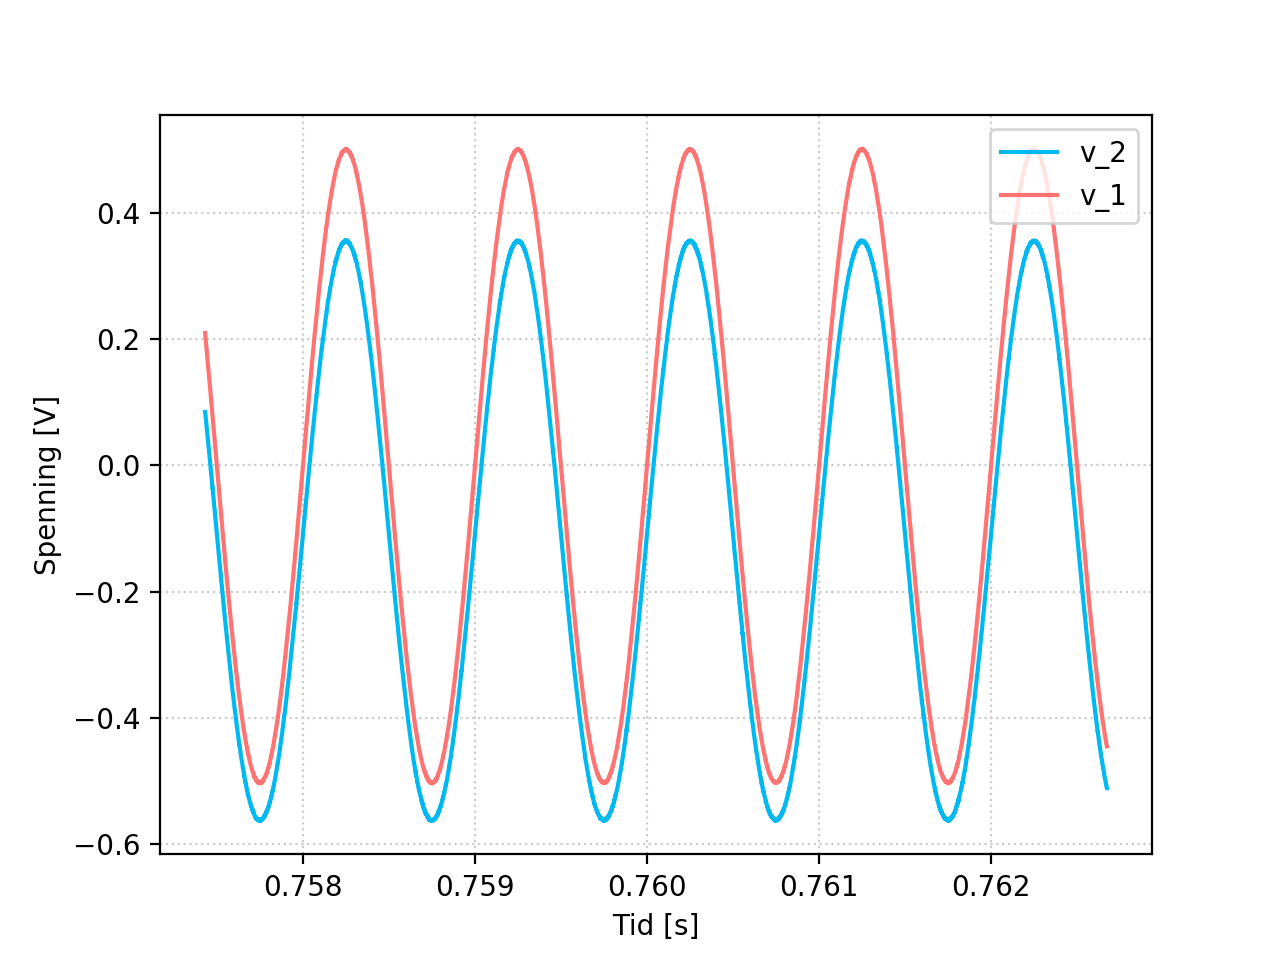
\includegraphics[width=0.8\textwidth]{img/reell-last-kilde.png}
    \caption{Systemet med realistisk last og kilde.}
    \label{fig:real}
\end{figure}
\vspace{1cm}

En finner at $A_2=458\text{mV}$ og $A_1=500\text{mV}$, som vil si at $v_2\approx v_1$, og systemet funker for en reell last og kilde. Den fysiske implementasjonen av kretsen, med reell last og kilde, vises i figur \ref{fig:real-circuit}.

\vspace{1cm}
\begin{figure}[!h]
    \centering
    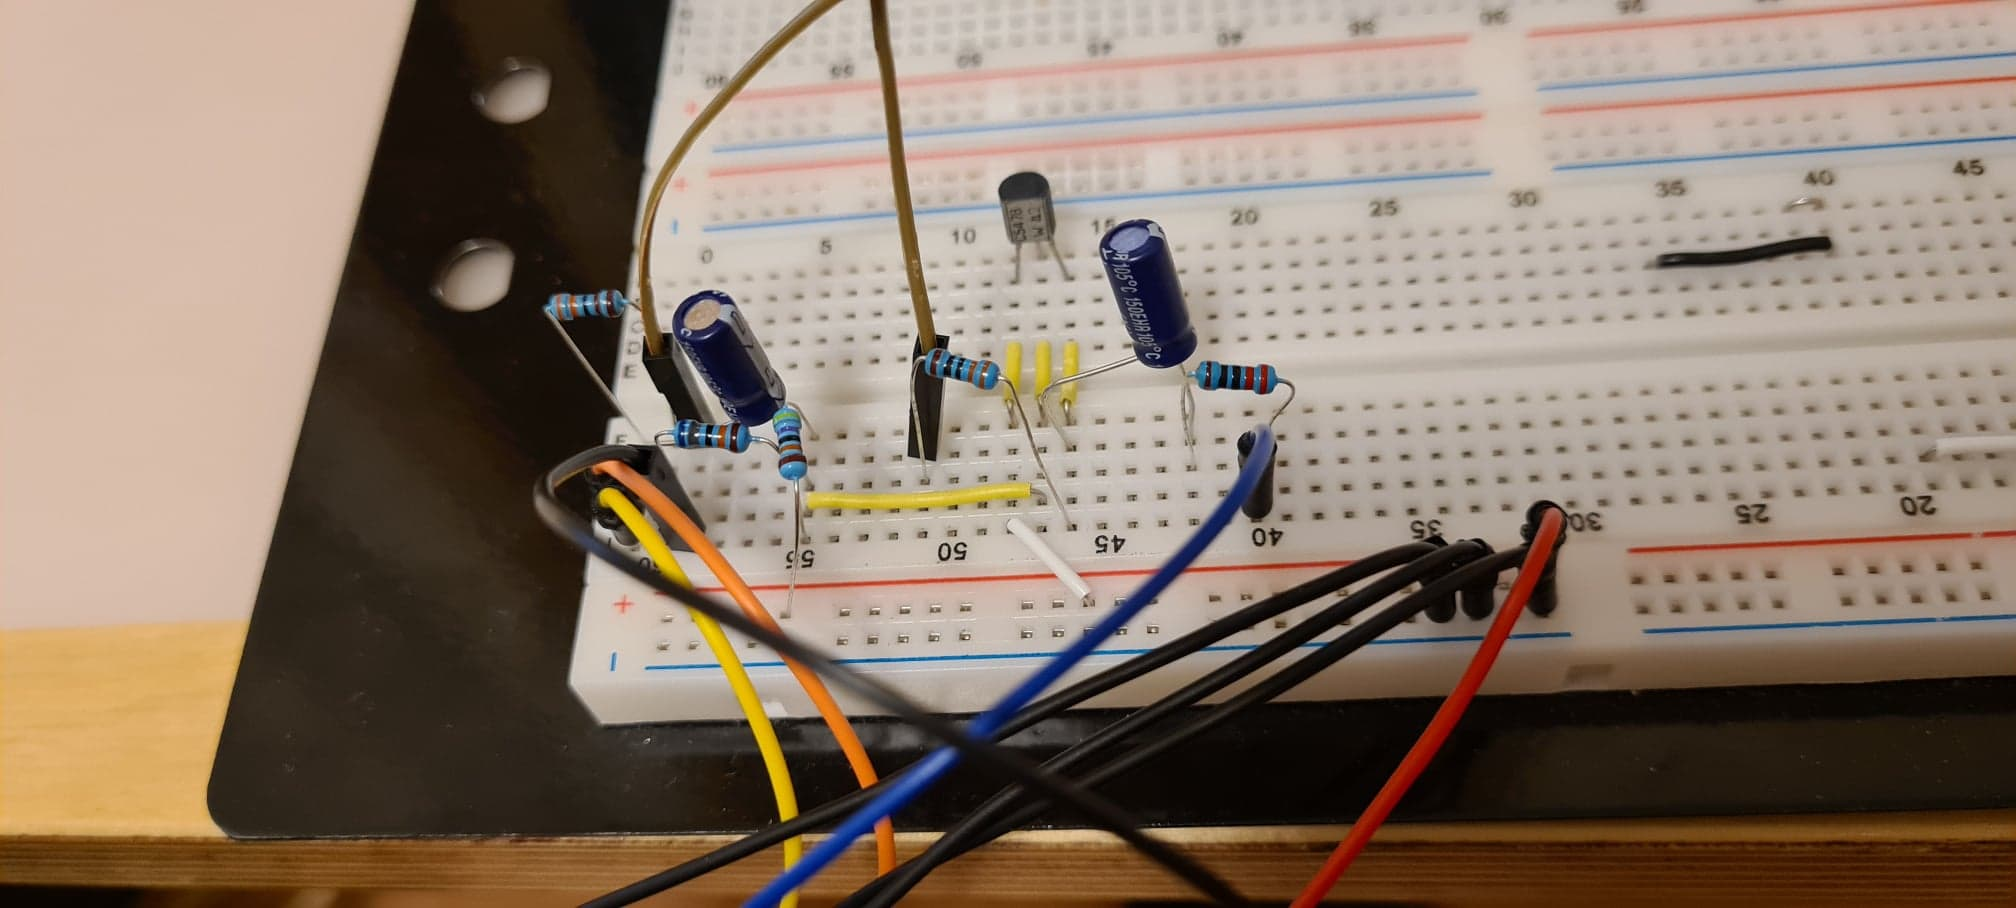
\includegraphics[width=\textwidth]{img/119455020_3605124586185980_8976253010718534837_n.jpg}
    \caption{Det realiserte systemet med realistisk last og kilde.}
    \label{fig:real-circuit}
\end{figure}
\vspace{1cm}

\clearpage


\subsection{Diskusjon}
Systemet ble testa for hvor stor amplitude $v_0$ kan ha før $v_2$ ble klippa, og resultatet vises i figur \ref{fig:v0max}. Der finner en at når $A_1=1\text{V}$, så klippes $v_2$ til $A_2=828\text{mV}$.

\vspace{1cm}
\vspace{1cm}
\begin{figure}[!h]
    \centering
    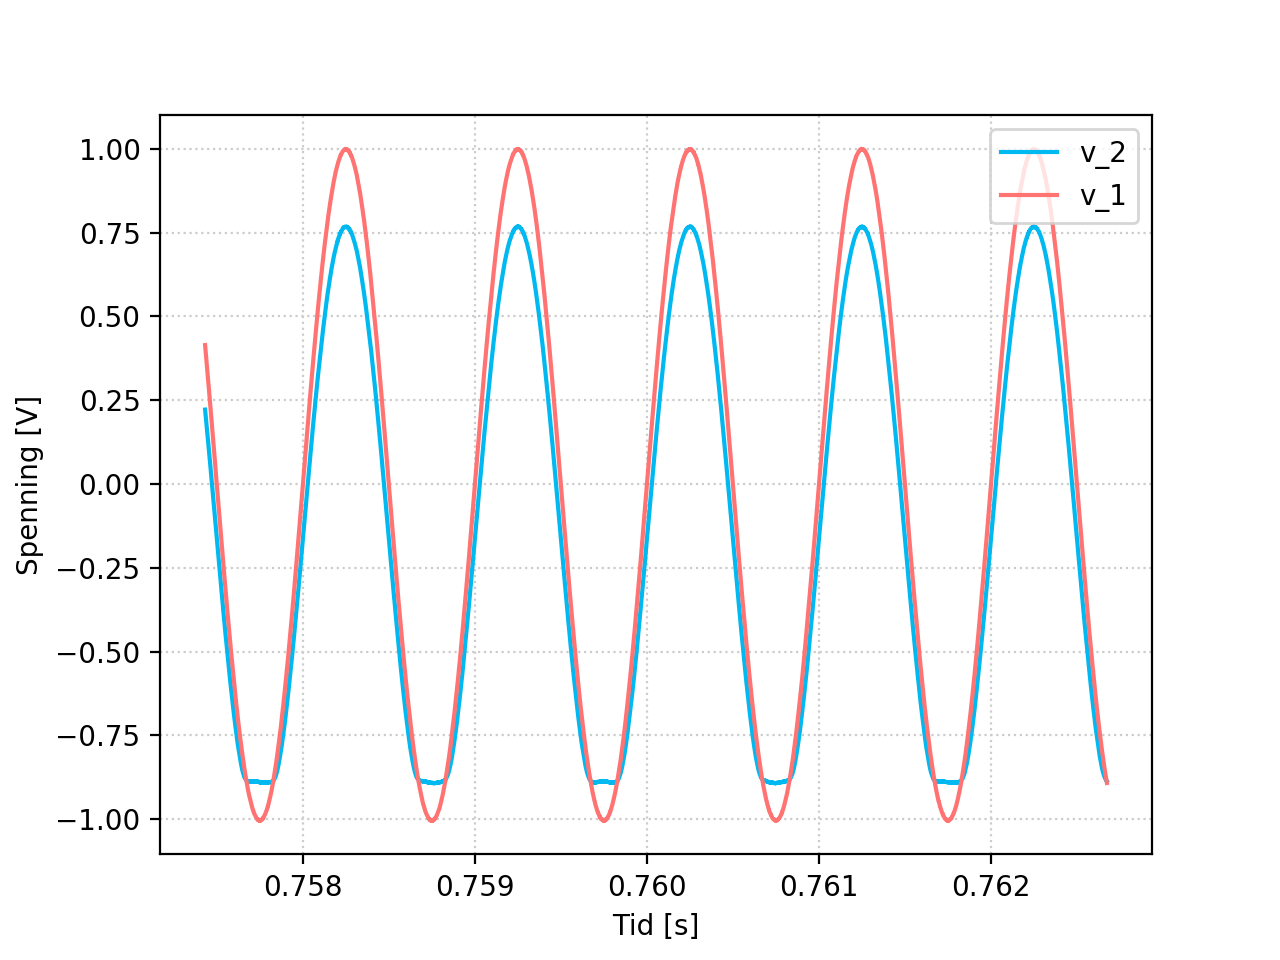
\includegraphics[width=0.8\textwidth]{img/v0max.png}
    \caption{Maksimal amplitude av $v_0$ før $v_2$ klippes.}
    \label{fig:v0max}
\end{figure}
\vspace{1cm}

Verdiene for $R_{\text{B}1}$ og $R_{\text{B}2}$ bestemmer hvor godt systemet funker som en buffer. For at en buffer skal fungere korrekt, så må inngangsimpedansen være høy, og utgangsimpedansen være lav. Verdiene for kondensatorene trenger kun å være tilstrekkelig store i forhold til systemet, og de vil fungere som kortslutninger i en småsignalanalyse (som ikke ble gjort for dette systemet, da en ikke trenger det for å beregne nødvendige komponentverdier).


Frekvensresponsen til systemet vises i figuren under, og en finner at knekkfrekvensen er ved ca. $2\text{MHz}$.

\vspace{1cm}
\begin{figure}[!h]
    \centering
    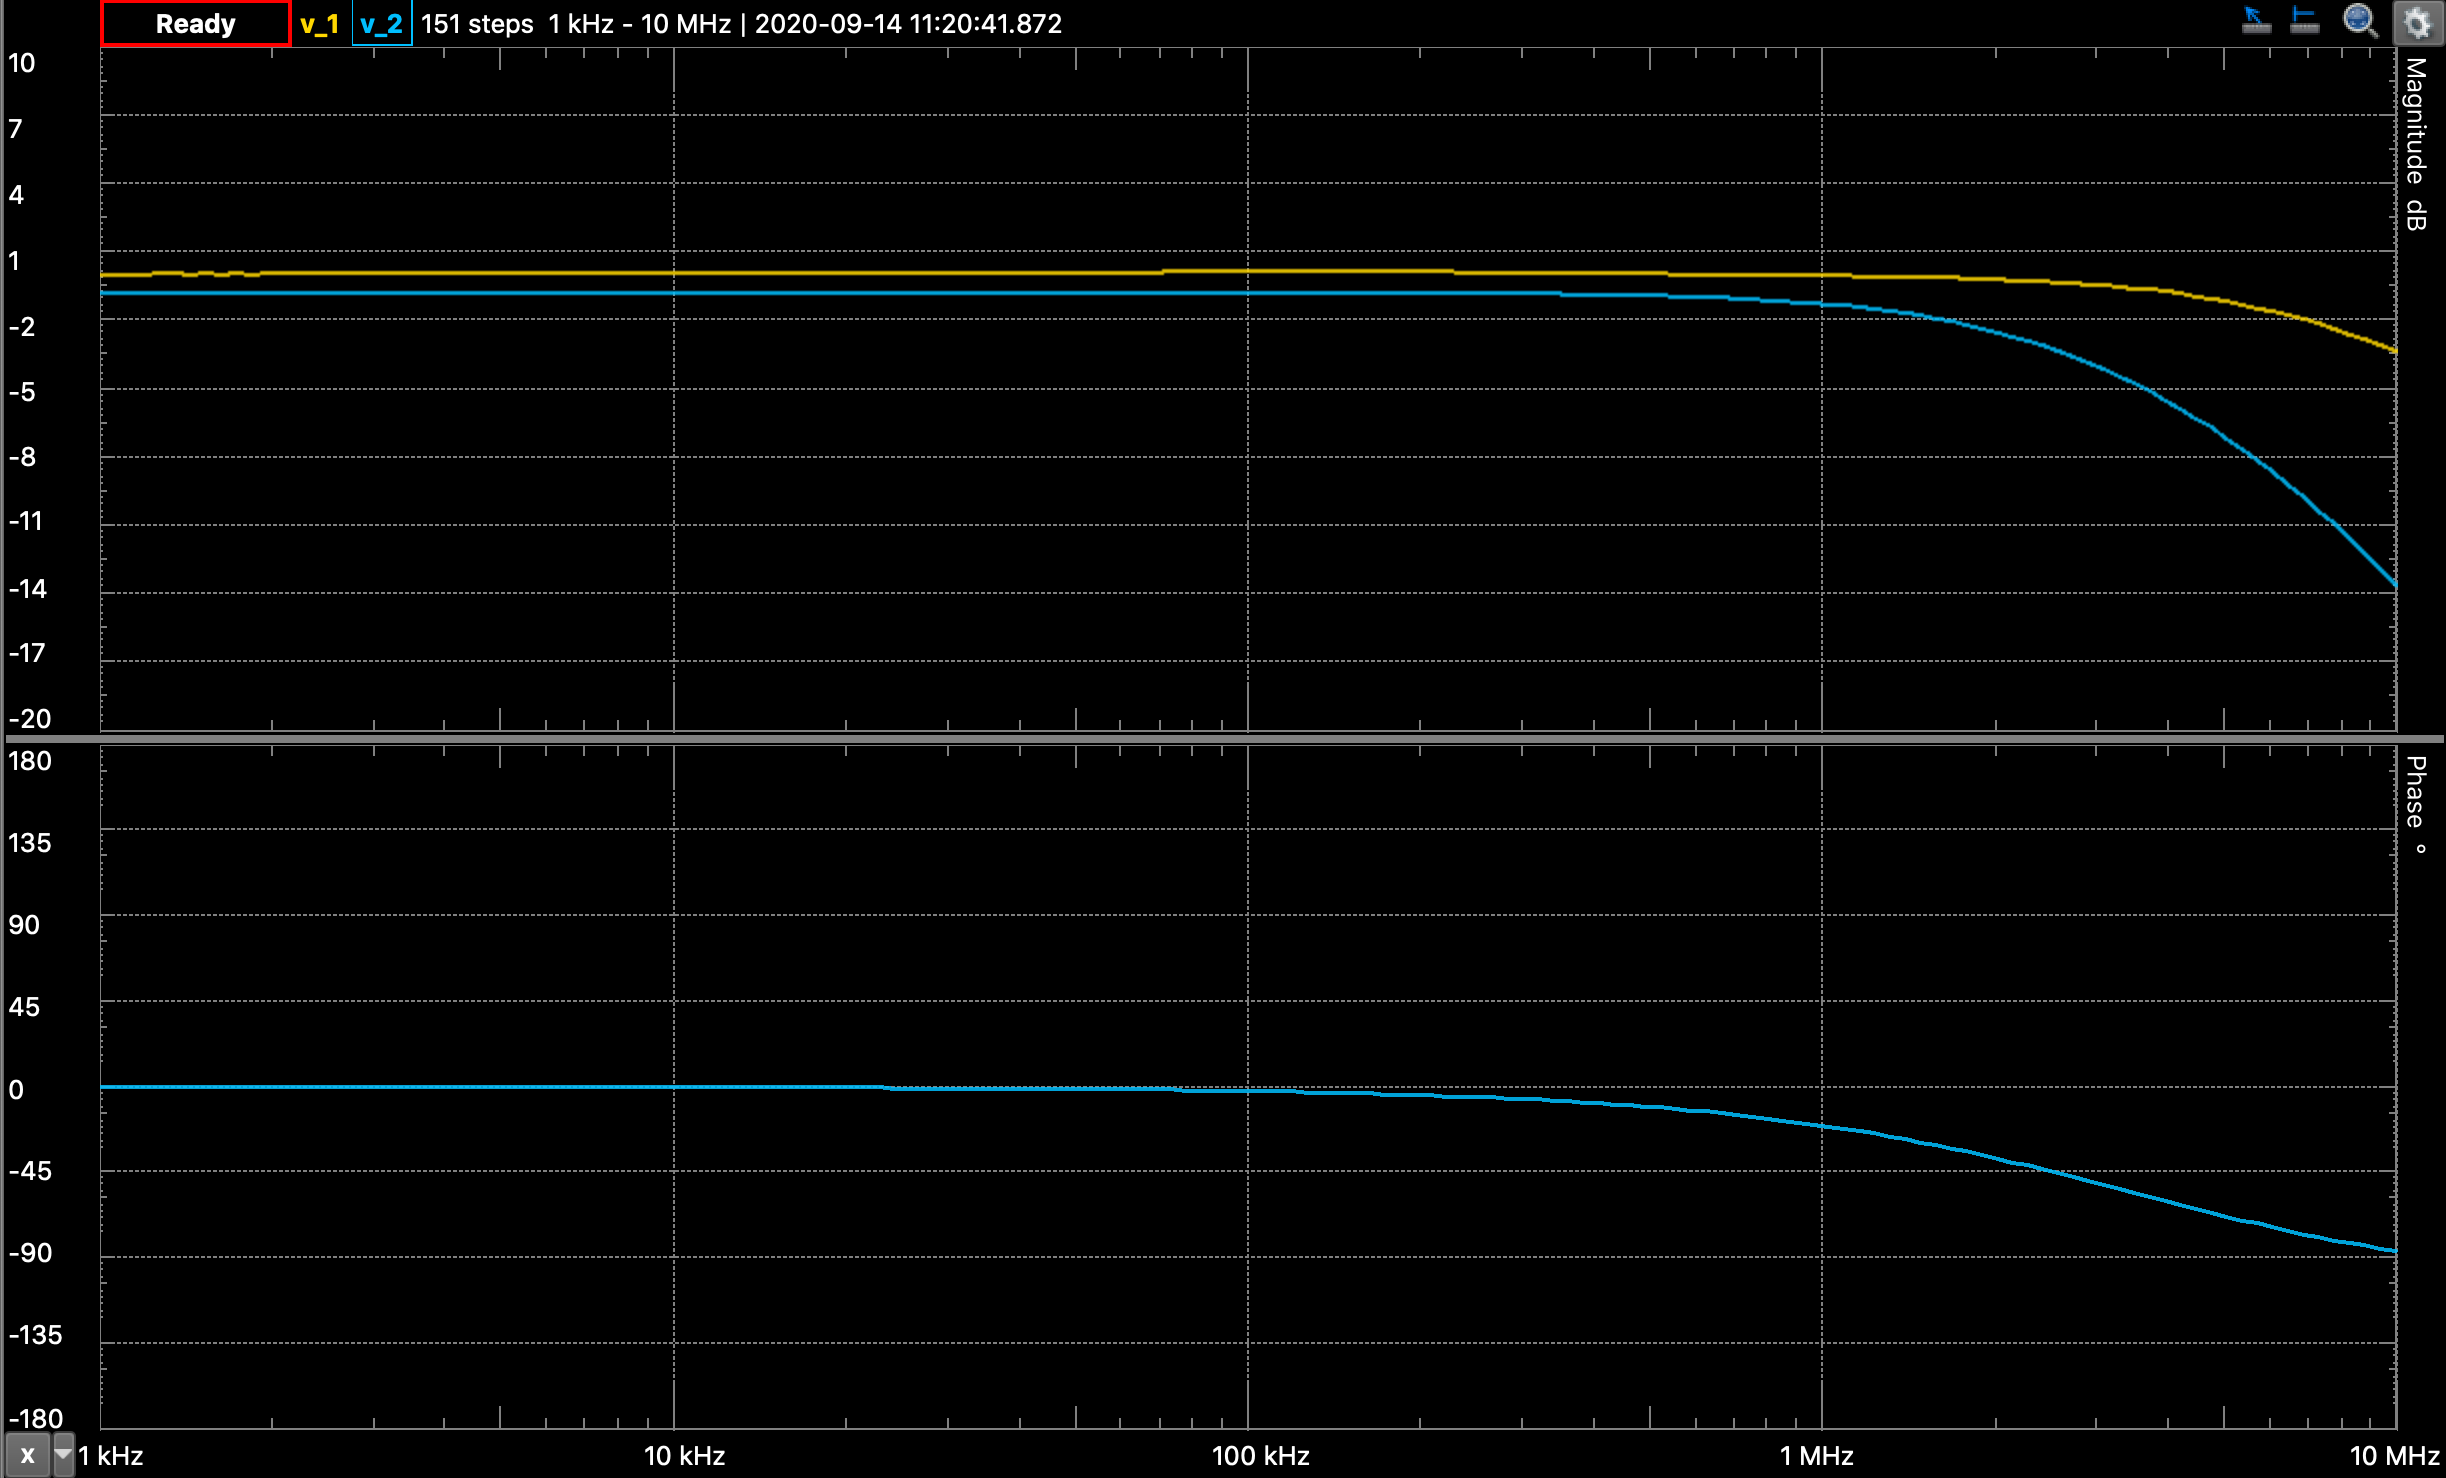
\includegraphics[width=1\textwidth]{img/frekvens-d5.png}
    \caption{Systemets frekvensrespons.}
    \label{fig:f}
\end{figure}
\vspace{1cm}\clearpage
\section{Konklusjon}
\label{sec:konklusjon}

For å løse problemet ved at et system ikke har en inngangskilde som kan levere nok strøm til en last, så kan en bruke en buffer. Et mulig design for dette vises i figur \ref{fig:02} og er blitt testa under ideelle og realistiske forhold. En finner at systemet fungerer godt under begge forhold, og utgangssignalet klippes når inngangssignalet er f.o.m $1\text{V}$. For å konkludere, så vil dette systemet gi $v_2\approx v_1\approx v_0$, og systemet fungerer godt.\clearpage
\section{Takk}
Takk til Stud. Marie Eriksen Grude, Stud. Anders Lundberg, Stud. Mathias Støle  og Stud. Sivert Sivertsen for godt samarbeid og nyttige diskusjoner om både teori og praktisk implementering av designprosjektet.\clearpage




%Bibliografi: Legg til flere elementer ved å legge til flere \bibitem:--------
\phantomsection
\addcontentsline{toc}{section}{Referanser}
\begin{thebibliography}{99}
  
\bibitem{buffer}
    Learning About Electronics,
    \emph{How to Build a Buffer Circuit with a Transistor},
    \url{http://www.learningaboutelectronics.com/Articles/Transistor-buffer-circuit.php},
    2018.

\end{thebibliography}


\newpage



\appendix
%Tillegg. Flere tillegg legges til ved å lage flere sections:-----------------
\section{Fullstendige utregninger}\label{ax:math}

\subsection{Bestemmelse av komponentverdier}

\begin{equation}
    \label{eq:arbeidspunkt}
    \begin{split}
    V_B &= \frac{V_{CC} - V_{BE}}{2} + V_{BE}\\
    V_B &= \frac{7V - 1,4V}{2} + 1,4V = 4.2V
    \end{split}
    \end{equation}
    
    \begin{equation}
    \label{eq:IE}
    \begin{split}
    I_{E1} &= I_{C1} + I_{B}\\
    I_{E1} &= I_{B}(\beta + 1)\\
    I_{E} &= I_{C2} + I_{E1}\\
    I_{E} &= I_{B}(\beta + 1)^2 \\
    \end{split}
    \end{equation}
    
    \begin{equation}
    \label{eq:IB}
    \begin{split}
    I_{B} &= \frac{I_{E}}{(\beta + 1)^2} \\
    I_{B} &= \frac{50mA}{(330 + 1)^2} = 0.45\mu A
    \end{split}
    \end{equation}
    
    \begin{equation}
    \label{eq:R1}
    \begin{split}
    R_{1} &= \frac{V_{CC} - V_{B}}{I_{B}}\\
    R_{1} &= \frac{7V - 4.2V}{1000*0.45\mu A} = 6.2k\Omega
    \end{split}
    \end{equation}
    
    \begin{equation}
    \label{eq:R2}
    \begin{split}
    V_{R2} &= \frac{V_{CC} R_2}{R_1 + R_2}\\
    R_2 &= \frac{V_{R2} R_1}{V_{CC}-V_{R2}}\\
    R_2 &= \frac{4.2V 6.2k\Omega}{7V-4.2V} = 9.3k\Omega
    \end{split}
    \end{equation}
    
    \begin{equation}
    \label{eq:RE}
    \begin{split}
    R_{E} &= \frac{V_{B}}{I_{E}}?\\ 
    \end{split}
    \end{equation}
    
    

\end{document}